\chapter{Część techniczna/praktyczna}
\section{Rozpoznawanie dłoni}

\quad Pierwszym elementem projektu jest rozpoznanie dłoni poprzez wyznacznie pozycji elementów charakterystycznych. Pozycja każdego z tych elementów jest względna wedłgu pozycji nadgarstka. ????



\subsection{Elementy charakterystyczne}

\quad Model modułu MediaPipe pozwala na wyznaczenie pozycji 21 elementów charakterystycznych dłoni. Współrzędne X i Y są znomralizowane względem rozdzielczości obrazu kamery. Współrzędna X względem liczby pikseli w osi X, a współrzędna Y względem liczby pikseli w osi Y. Oś Z jest prostopadła do osi X i Y, z punktem początkowym w punkcie określającym pozycję nadgarstka. Współrzędna Z jest znormalizowana względem szerokości obrazu kamery, tak jak współrzędna X. 

\begin{figure}[H]
\begin{center}
    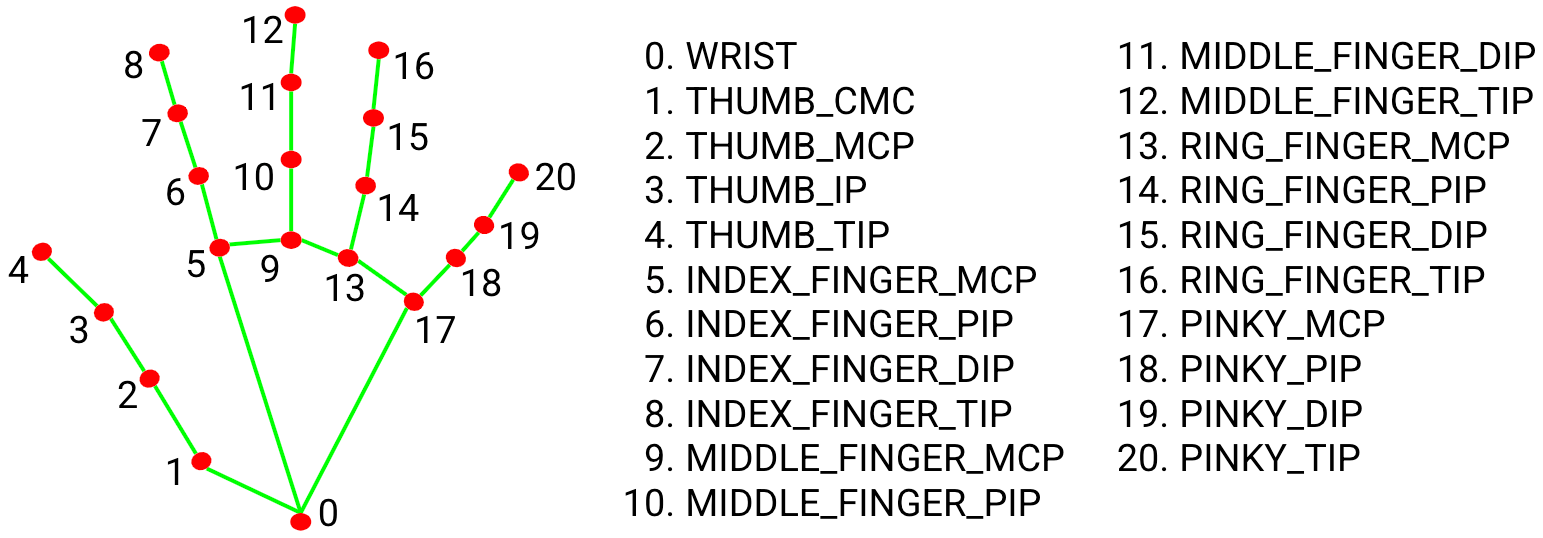
\includegraphics[width=15cm]{hand_landmarks.png}
    \caption{Elementy charakterystyczne dłoni}
\end{center}
\end{figure}

\quad Pozycje nadgarstka, paliczków oraz stawów dłoni zostaną wykorzystane do obliczenia obrotu dłoni względem punkut 0 oraz do wytrenowania modeli uczenia maszynowego, których zadaniem będzie rozpoznawnie wybranych gestów. 

\newpage
\subsection{OpenCV - przygotowanie obrazu z kamery}

\quad Poprawne działanie modelu MediaPipe wymaga odpowiedniego przygotowania obrazu kamery. Działanie kontrolerolera odbywa się poprzez główną metodę \textbf{main()}.

Metoda \textbf{main()} jest główną funkcją, w której dokonywane są obliczenia oraz przeszktałcenia pozwalające na obliczenie obrotu dłonie, odległości między wybranymi palcami oraz na wykrycie gestu. 

\inputminted[firstline=51, lastline=52]{python}{../OpenLeap.py}

\quad W pierwszym kroku tworzymy instancję klasy \textbf{VideoCapture} biblioteki \textbf{OpenCV}, która pozwoli na odczytywanie obrazu kamery. 

\inputminted[firstline=272, lastline=297]{python}{../OpenLeap.py}


\quad tekst testowy

\subsection{Generowanie grafiki dłoni}

\section{SciKit Learn - uczenie maszynowe}
\subsection{Budowa programu}
\subsection{Zebranie danych}
\subsection{Metody klasyfikacji - uczenie maszynowe}
\subsection{Ponowne wykorzystanie modelu}

\section{Paczka PyPi}
\subsection{Budowa paczki}
\subsection{Plik setup.py}
\subsection{Załadowanie paczki do repozytorium}
